
\documentclass[a4paper,11pt]{article}%,twocolumn
%% packages

\usepackage{blindtext} % needed for creating dummy text passages
%\usepackage{ngerman} % needed for German default language
\usepackage{amsmath} % needed for command eqref
\usepackage{amssymb} % needed for math fonts
\usepackage[colorlinks=true,breaklinks]{hyperref} % needed for creating hyperlinks in the document, the option colorlinks=true gets rid of the awful boxes, breaklinks breaks lonkg links (list of figures), and ngerman sets everything for german as default hyperlinks language
\usepackage[hyphenbreaks]{breakurl} % ben�tigt f�r das Brechen von URLs in Literaturreferenzen, hyphenbreaks auch bei links, die �ber eine Seite gehen (mit hyphenation).
\usepackage{xcolor}
\definecolor{c1}{rgb}{0,0,1} % blue
\definecolor{c2}{rgb}{0,0.3,0.9} % light blue
\definecolor{c3}{rgb}{0.3,0,0.9} % red blue
\hypersetup{
    linkcolor={c1}, % internal links
    citecolor={c2}, % citations
    urlcolor={c3} % external links/urls
}
%\usepackage{cite} % needed for cite
\usepackage[square,authoryear]{natbib} % needed for cite and abbrvnat bibliography style
\usepackage[nottoc]{tocbibind} % needed for displaying bibliography and other in the table of contents
\usepackage{graphicx} % needed for \includegraphics 
\usepackage{longtable} % needed for long tables over pages
\usepackage{bigstrut} % needed for the command \bigstrut
\usepackage{enumerate} % needed for some options in enumerate
%\usepackage{todonotes} % needed for todos
\usepackage{makeidx} % needed for creating an index
\makeindex
\usepackage{gensymb}
\usepackage{url}
\usepackage{psfrag}
\usepackage{multirow}
\usepackage{subfigure}
%% page settings

\usepackage[top=20mm, bottom=20mm,left=15mm,right=15mm]{geometry} % needed for page border settings
\parindent=0mm % for space of first line of new text block
\sloppy % for writing with hyphenless justification (tries to)
\hyphenation{} % use hyphenation of tolerance parametershttp://www.jr-x.de/publikationen/latex/tipps/zeilenumbruch.html
\hyphenpenalty=10000
\exhyphenpenalty=10000
\usepackage{fancyhdr} % needed for head and foot options
%% my macros

%% Text fomats
\newcommand{\tbi}[1]{\textbf{\textit{#1}}}

%% Math fonts
\newcommand{\bbA}{\mathbb{A}}
\newcommand{\bbB}{\mathbb{B}}
\newcommand{\bbC}{\mathbb{C}}
\newcommand{\bbD}{\mathbb{D}}
\newcommand{\bbE}{\mathbb{E}}
\newcommand{\bbF}{\mathbb{F}}
\newcommand{\bbG}{\mathbb{G}}
\newcommand{\bbH}{\mathbb{H}}
\newcommand{\bbI}{\mathbb{I}}
\newcommand{\bbJ}{\mathbb{J}}
\newcommand{\bbK}{\mathbb{K}}
\newcommand{\bbL}{\mathbb{L}}
\newcommand{\bbM}{\mathbb{M}}
\newcommand{\bbN}{\mathbb{N}}
\newcommand{\bbO}{\mathbb{O}}
\newcommand{\bbP}{\mathbb{P}}
\newcommand{\bbQ}{\mathbb{Q}}
\newcommand{\bbR}{\mathbb{R}}
\newcommand{\bbS}{\mathbb{S}}
\newcommand{\bbT}{\mathbb{T}}
\newcommand{\bbU}{\mathbb{U}}
\newcommand{\bbV}{\mathbb{V}}
\newcommand{\bbW}{\mathbb{W}}
\newcommand{\bbX}{\mathbb{X}}
\newcommand{\bbY}{\mathbb{Y}}
\newcommand{\bbZ}{\mathbb{Z}}
\usepackage[ framed, numbered]{matlab-prettifier}%framed,%
\usepackage{listings}
\usepackage{physics}
\usepackage{pdfpages}
\usepackage[toc,page]{appendix}
\usepackage{float}
\usepackage{hyperref}

\newenvironment{qanda}{\setlength{\parindent}{0pt}}{\bigskip}
\newcommand{\Q}{\bigskip\bfseries Q: }
\newcommand{\A}{\par\textbf{Answer: } \normalfont}

\begin{document}
\begin{titlepage}
\center % Center everything on the page

%-------------------------------------------------------------------------------------
%	HEADING SECTIONS
%------------------------------------------------------------------------------------
\textbf{\large Department of Electrical and Computer Engineering}\\[0.5cm]
\textbf{\Large University of Colorado at Boulder}\\[1cm]
\textbf{\large ECEN5623 - Real Time Embedded Systems }\\[2cm]

\includegraphics[width=0.3\textwidth]{figures/cu}\\[2cm]

	
%-------------------------------------------------------------------------------------
%	TITLE SECTION
%------------------------------------------------------------------------------------
\textbf{\Huge Exercise 5 }\\[0.2cm]



%----------------------------------------------------------------------------------------
%	MEMBERS SECTION
%----------------------------------------------------------------------------------------


\vfill

\textbf{\large Submitted by}\\[0.5cm]

{\large Parth | Jithedra}\\[0.5cm]	

%----------------------------------------------------------------------------------------
%	DATE SECTION
%----------------------------------------------------------------------------------------

\textbf{\large Submitted on}
\textbf{\Large \today} % Date, change the \today to a set date if you want to be precise

%----------------------------------------------------------------------------------------

\vfill % Fill the rest of the page with whitespace

\end{titlepage}


\pagebreak

\tableofcontents
\listoffigures
\listoftables
\vfill
\begin{center}
	\textbf{\textit{*PDF is clickable}}
\end{center}

\pagebreak



\begin{qanda}

	\section{Question 1}
	\Q  Implement a Linux process that is executed at the default priority for a user-level application and waits on a binary semaphore to be given by another application. Run this process and verify its state using the ps command to list its process descriptor. Now, run a separate process to give the semaphore causing the first process to continue execution and exit. Verify completion.
	\addcontentsline{toc}{subsection}{Answer}
	\A
	I wrote a C program named sem\_wait that waits for a semaphore to be signaled by another program. Additionally, I wrote another C program called sem\_post that signals this semaphore. Below are the steps and screenshots demonstrating the waiting program until the semaphore is signaled.

	here are steps for to run semaphore programs
	\begin{enumerate}
		\item First, I executed the sem\_wait program. This program will wait for a semaphore signal. A screenshot confirms the program is in a wait state.

		      \begin{figure}[!h]
			      \centering
			      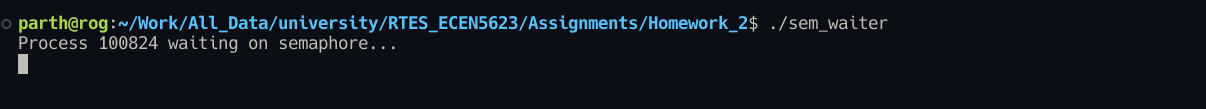
\includegraphics[scale=0.6]{figures/sem_waiter.png}
			      \caption{Program is running and is in wait state}
		      \end{figure}
		\item Using the ps command, I checked that the sem\_wait program is indeed running and has not completed its execution. This is shown in the screenshot below.
		      \begin{figure}[!h]
			      \centering
			      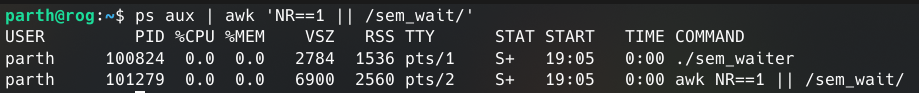
\includegraphics[scale=0.6]{figures/ps_sem_waiter.png}
			      \caption{PS command that shows that our program is waiting for semaphore}

		      \end{figure}
		\item Next, I ran the sem\_post program, which signals the semaphore for the waiting program.
		      \begin{figure}[!h]
			      \centering
			      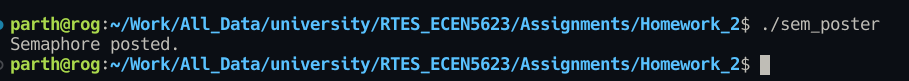
\includegraphics[scale=0.6]{figures/sem_poster.png}
			      \caption{Semaphore has been posted by this program}

		      \end{figure}

		\item After the semaphore was signaled, the sem\_wait program completed its execution. This is evident from the following screenshot.
		      \begin{figure}[!h]
			      \centering
			      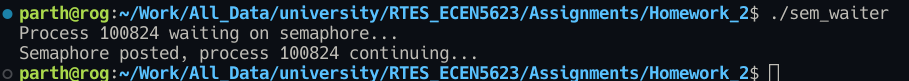
\includegraphics[scale=0.6]{figures/sem_waiter_complete.png}
			      \caption{Output of program waiting for semaphore}

		      \end{figure}

		\item Lastly, I used the ps command again to verify that the waiting program had indeed completed after the semaphore was posted. The screenshot intended to show this step appears to be repeated from step 4. It should ideally confirm the waiting program's completion.
		      \begin{figure}[!h]
			      \centering
			      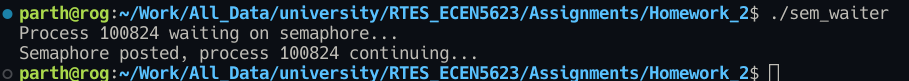
\includegraphics[scale=0.6]{figures/sem_waiter_complete.png}
			      \caption{PS output after Semaphore posted}

		      \end{figure}

	\end{enumerate}

	Through these steps and screenshots, it's demonstrated how one program can wait for a semaphore to be signaled by another, showcasing basic inter-process communication and synchronization in Linux.



	\section{Question 2}
	\Q   If EDF can be shown to meet deadlines and potentially has 100\% CPU resource utilization, then why is it not typically the hard real-time policy of choice? That is, what are drawbacks to using EDF compared to	RM/DM? In an overload situation, how will EDF fail?
	\addcontentsline{toc}{subsection}{Answer}
	\A

	\textbf{Drawbacks of EDF Compared to RM/DM}
	\begin{enumerate}
		\item \textbf{Sensitivity to Task Overruns:} In EDF scheduling, if a task overruns its expected execution time, it can lead to a domino effect where subsequent tasks also miss their deadlines. This is because EDF always prioritizes the task with the closest deadline, meaning an overrunning task continues to preempt others, potentially leading all tasks in the queue to miss their deadlines.
		\item \textbf{Complexity in Handling New Tasks:} Adding a new task to the queue requires adjusting priorities across all tasks. If there's an overrunning task, it won't be preempted by newly added tasks, even if they have sooner deadlines, because the overrunning task has a 'negative' time to its deadline, keeping it at the highest priority.
		\item \textbf{Difficulty in Overrun Detection and Management:} Managing task overruns in EDF requires detecting the overrun and potentially terminating the overrunning task. This process itself consumes CPU resources, which can further compromise the system's ability to meet deadlines, especially without any margin for error.
		\item \textbf{Challenges in Predicting Affected Services:} In overload scenarios, while EDF's adjustment to focus on tasks with the soonest deadlines seems logical, predicting which tasks will fail to meet their deadlines due to dynamic releases and priority adjustments is difficult.
	\end{enumerate}







	\textbf{EDF Failure in Overload Situations}
	In an overload scenario, EDF can lead to a cascading failure where multiple services miss their deadlines because of a single overrunning service. This failure mode is more severe in EDF compared to RM or DM because RM/DM schedules are static and prioritize tasks based on their fixed rates or deadlines, not dynamically adjusting to the current load or task overruns. This makes RM/DM potentially more predictable and stable under overload conditions, even if they might not utilize CPU resources as efficiently as EDF under normal conditions.\\

	The book by sam siewert suggests that, in the face of an overload, the best course of action for an EDF scheduler might be to drop all services in the queue, aiming for a more deterministic outcome. While this approach ensures predictability, it also indicates a significant limitation of EDF in handling overloads effectively without compromising system reliability.\\

	In summary, while EDF can theoretically achieve 100\% CPU utilization and meet deadlines under ideal conditions, its sensitivity to task overruns, complexity in handling dynamic priority adjustments, and challenges in managing overload situations make it less desirable for hard real-time systems compared to RM or DM. RM and DM's predictability and stability, even at the cost of potentially lower CPU utilization, are often more critical in environments where meeting every deadline is paramount.
	\pagebreak
	\section{Question 3}
	\Q   If a system must complete frame processing so that 100,000 frames are completed per second and the instruction count per frame processed is 2,120 instructions on a 1 GHz processor core, what is the CPI	required for this system? What is the overlap between instructions and IO time if the intermediate IO time is
	4.5 microseconds?
	\addcontentsline{toc}{subsection}{Answer}
	\A
	The total number of instructions processed per second is the product of the frame processing rate and the instruction count per frame. The CPI (Cycles Per Instruction) can then be determined by dividing the total number of cycles available per second by the total number of instructions processed per second.

	\begin{flalign*}
		 & Instructions\_per\_second = Frame\_processing\_rate \cdot Instruction\_per\_frame &  & \\
		 & Instructions\_per\_second = 10000 \cdot 2120                                      &  & \\
		 & \boxed{Instructions\_per\_second = 21200000}                                      &  & \\\\
		 & \text{Now for CPI}                                                                &  & \\
		 & CPI = \frac{Clock\_speed}{Instructions\_per\_second}                              &  & \\
		 & CPI = \frac{1 \cdot 10^{9}}{21200000}                                             &  & \\
		 & \boxed{CPI = 4.71698 \quad C/I}                                                   &  & \\
	\end{flalign*}

	\textbf{Overlap Calculation}
	The overlap between instructions and I/O time can be considered as the time during which the processor can perform other tasks while waiting for I/O operations to complete. Given the intermediate I/O time, we can calculate the amount of overlap by considering the total time available for processing each frame and the I/O time.

	The instruction execution time would be\\

	\begin{flalign*}
		& Instruction\_execution\_time = \frac{Instruction\_per\_frame \cdot CPI}{Processor\_clock} &  & \\
		& Instruction\_execution\_time = \frac{2120 \cdot 4.71698}{10^{9}} &  & \\
		& \boxed{Instruction\_execution\_time = 1 \cdot 10^{-5} \quad sec}                             &  & \\
   \end{flalign*}

   And overlapping percentage would be\\
	\begin{flalign*}
		 & Overlap\_percentage = \frac{IO\_time}{Instruction\_execution\_time} \cdot 100 &  & \\
		 & Overlap\_percentage = \frac{4.5 \cdot 10^{-6}}{1 \cdot 10^{-5}} \cdot 100 &  & \\
		 & Overlap\_percentage = 0.45 \cdot 100 &  & \\
		 & \boxed{Overlap\_percentage = 45\%}                             &  & \\
	\end{flalign*}




\end{qanda}


\section{Referance}
\begin{enumerate}
	\item REAL-TIME EMBEDDED COMPONENTS AND SYSTEMS with LINUX and RTOS by Sam Siewert John Pratt
	\item Scheduling Algorithms for Multiprogramming in a Hard Real-Time Environment C. L. LIU AND JAMES W. LAYLAND
	\item https://bears.ece.ucsb.edu/class/ece253/lect7.pdf
\end{enumerate}


\vfill
\hrule
\vspace{0.5cm}

\begin{appendices}
	\section{C Code for the Implementation}
	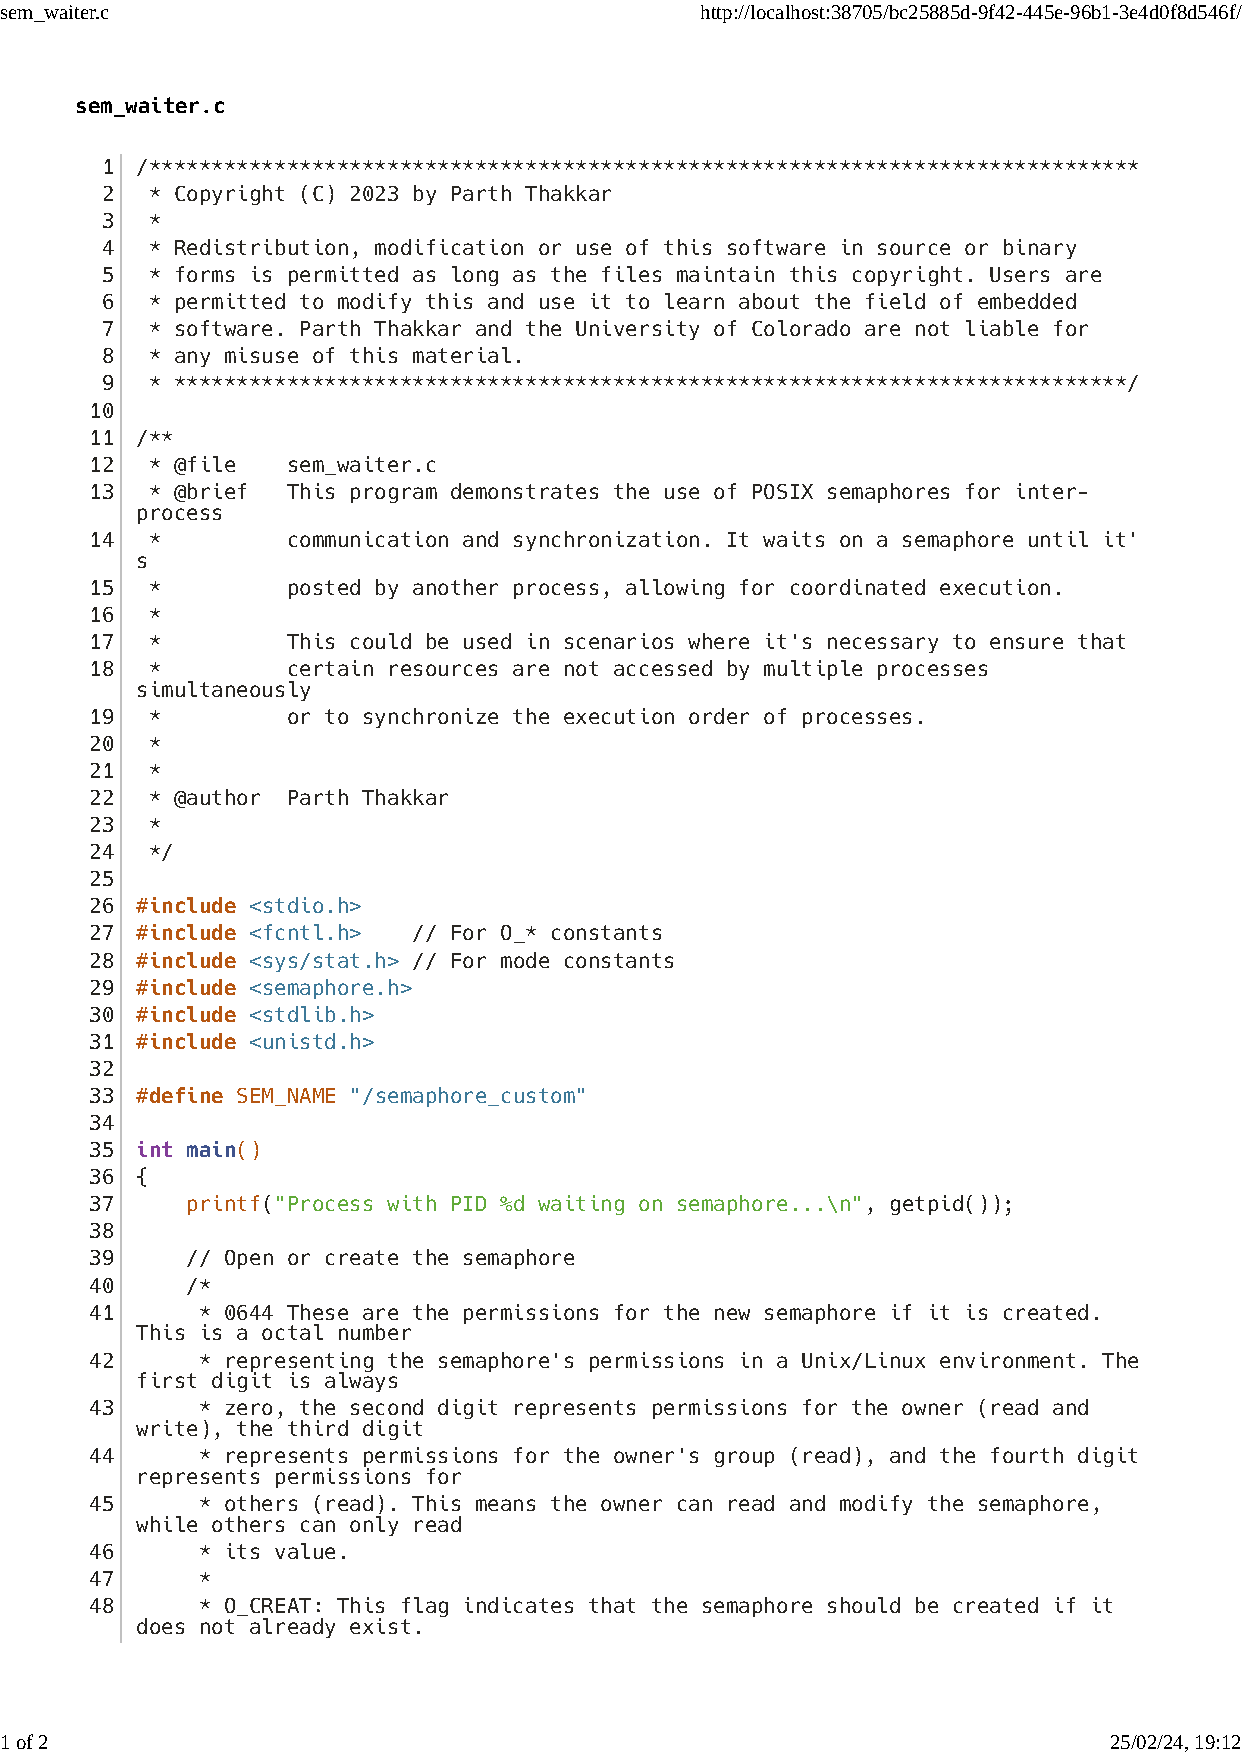
\includepdf[pages=-]{code/sem_waiter.c.pdf}

	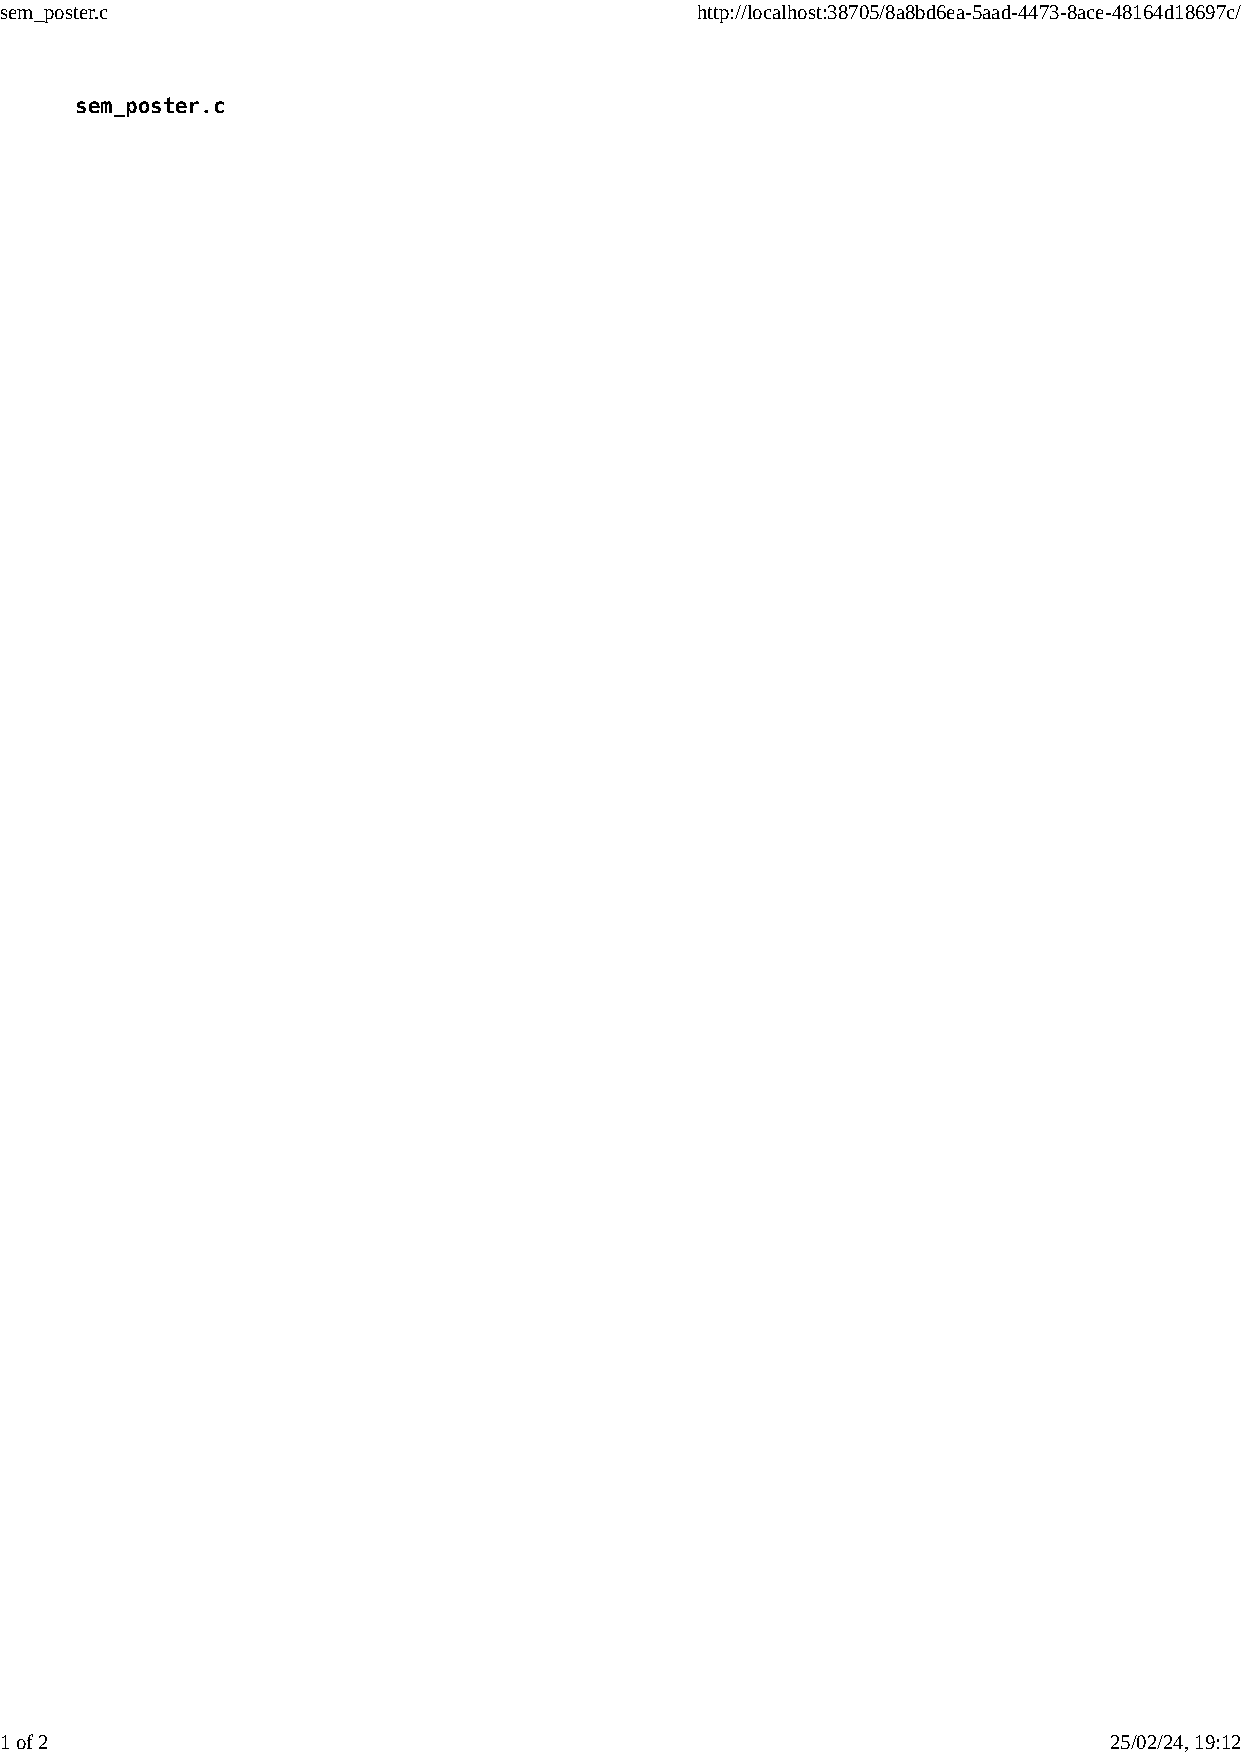
\includepdf[pages=-]{code/sem_poster.c.pdf}
\end{appendices}


\vspace{1cm}
\hrule
\vspace{0.5cm}


%---------------------------------------------------------------------------
\end{document}
-
